% -*- root: ../../DAT2-A423_Project_Report.tex -*-
\section{Using the Graph Theoretical Approach on JPEG images}
In section \ref{sec:graphtheory} we took a closer look on the Graph-Theoretic Approach for Steganography. The goal of this section is to understand how we can modify the technique to work on JPEG images instead of grey-scale Bitmap images. The authors of the method defines the following about using the technique on JPEG images\cite{hetzl_2005}:

\begin{itemize}
	\item The samples (i.e. where the data will be embedded) are the coefficients of the DCT operation. 
	\item The DC component must not be used for embedding data, as these are often large numbers and and would result in visible distortion of the image, if those were to be switched.
	\item AC components with a value of 0 must not be used for embedding data. If they were to be used, the Run/Length encoding step would be useless, as there will be very few zeroes in a row.
\end{itemize}

The process of encoding a JPEG image can be seen on figure \ref{fig:JPEGprocess}. Drawn onto the figure is also the embedding step, which will take place after the quantization process.

\begin{figure}[h!]
	\centering
	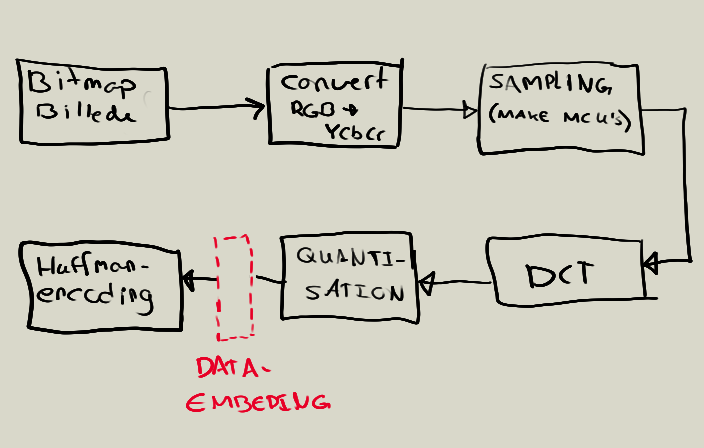
\includegraphics[width=0.95\textwidth]{figures/JPEGprocess.png}
	\caption{caption}
	\label{fig:JPEGprocess}
\end{figure}

There are two ways to go about encoding the message in the quantization coefficients. We could either create a graph for each 8x8 matrix of coefficients, or we combine all of the non-zero AC coefficients into an array and use these values to embed the message.